\documentclass[tikz,border=6pt]{standalone}
\usepackage{amsmath}
\usetikzlibrary{arrows.meta,calc}


\begin{document}
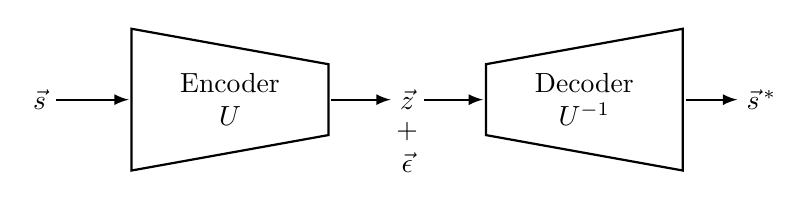
\begin{tikzpicture}[thick]

\typeout{IFSTANDALONE: \ifstandalone YES\else NO\fi}
\typeout{JOBNAME: \jobname}


\typeout{=== geo_autoencoder build ===}
\typeout{ENGINE: \ifluatex LuaLaTeX\else\ifxetex XeLaTeX\else pdfLaTeX\fi\fi}
\typeout{PGF: \pgfversion}
\makeatletter
\typeout{Latex tip defined? \ifcsname pgf@arrow@code@Latex\endcsname YES\else NO\fi}
\makeatother


% --------------------
% Parameters (tweak these)
% --------------------
\def\encL{18mm}   % encoder left height  (bigger)
\def\encS{9mm}    % encoder right height (smaller)
\def\blkW{25mm}   % block length
\def\gap{20mm}    % gaps between items
\def\portOff{3mm} % y-offset on the input edge for theta arrows
\def\nvoffset{4mm} % noise vec offset


% Derived lengths
\pgfmathsetlengthmacro{\encLh}{0.5*\encL}
\pgfmathsetlengthmacro{\encSh}{0.5*\encS}
\pgfmathsetlengthmacro{\blkWh}{0.5*\blkW}
\pgfmathsetlengthmacro{\halfgap}{0.5*\gap}
\pgfmathsetlengthmacro{\midgap}{1.2*\gap}

\tikzset{
  %arrow/.style={-{Latex[length=2.2mm]}, thick, shorten <=1pt, shorten >=1pt},
  arrow/.style={-latex, thick, shorten <=1pt, shorten >=1pt},
  vec/.style={draw=none, fill=white, rounded corners=2pt, inner sep=2pt}
}

% --------------------
% Vector nodes (borderless "boxes")
% --------------------
\node[vec] (x) at (0,0) {$\vec{s}$};

% --------------------
% Encoder trapezoid (left tall -> right short)
% --------------------
\coordinate (Ew) at ($(x.east)+(\halfgap,0)$);   % encoder input-edge midpoint
\coordinate (Ee) at ($(Ew)+(\blkW,0)$);         % encoder output-edge midpoint

\path[draw]
  ($(Ew)+(0,\encLh)$) --
  ($(Ew)+(\blkW,\encSh)$) --
  ($(Ew)+(\blkW,-\encSh)$) --
  ($(Ew)+(0,-\encLh)$) -- cycle;

\node[align=center] at ($(Ew)+(\blkWh,0)$) {Encoder\\$U$};

% --------------------
% Latent vector node
% --------------------
\node[vec] (z) at ($(Ee)+(\halfgap,0)$) {$\vec{z}$};
\node[align=center] (zp) at ($(z)-(0,\nvoffset)$) {+};
\node[align=center] at ($(zp)-(0,\nvoffset)$) {$\vec{\epsilon}$};

% --------------------
% Decoder trapezoid (left short -> right tall)
% --------------------
\coordinate (Dw) at ($(Ee)+(\gap,0)$);   % decoder input-edge midpoint
\coordinate (De) at ($(Dw)+(\blkW,0)$);         % decoder output-edge midpoint

\path[draw]
  ($(Dw)+(0,\encSh)$) --
  ($(Dw)+(\blkW,\encLh)$) --
  ($(Dw)+(\blkW,-\encLh)$) --
  ($(Dw)+(0,-\encSh)$) -- cycle;

\node[align=center] at ($(Dw)+(\blkWh,0)$) {Decoder\\$U^{-1}$};

% --------------------
% Output vector node
% --------------------
\node[vec] (xstar) at ($(De)+(\halfgap,0)$) {$\vec{s}^{\,*}$};

% --------------------
% Main dataflow arrows (use anchors so text isn't crossed)
% --------------------
\draw[arrow] (x.east) -- (Ew);
\draw[arrow] (Ee) -- (z.west);
\draw[arrow] (z.east) -- (Dw);
\draw[arrow] (De) -- (xstar.west);

\end{tikzpicture}
\end{document}
